% lecture02.tex: Lecture 2: Planet Formation 101 & Orbital Dynamics
% Introduction to Planetary Science, Kapteyn Institute

\documentclass[aspectratio=169, 11pt]{beamer}

% ── Theme and macros ────────────────────────────────────────
\usepackage{../common/beamerthemeIPS}
% macros.tex: Shared math macros for IPS lecture slides
% Mirrors definitions in book/_config.yml for consistency
% Uses \providecommand to avoid conflicts with unicode-math

% ── Derivatives ─────────────────────────────────────────────
\providecommand{\dv}[2]{\frac{\mathrm{d} #1}{\mathrm{d} #2}}
\providecommand{\dd}{}\renewcommand{\dd}{\mathrm{d}}
\providecommand{\pdv}[2]{\frac{\partial #1}{\partial #2}}

% ── Solar quantities ────────────────────────────────────────
\newcommand{\Msun}{M_{\odot}}
\newcommand{\Rsun}{R_{\odot}}
\newcommand{\Lsun}{L_{\odot}}

% ── Planetary quantities ────────────────────────────────────
\newcommand{\Mearth}{M_{\oplus}}
\newcommand{\Rearth}{R_{\oplus}}
\newcommand{\Mjup}{M_{\mathrm{J}}}
\newcommand{\Rjup}{R_{\mathrm{J}}}

% ── Constants ───────────────────────────────────────────────
\newcommand{\kB}{k_{\mathrm{B}}}

% ── Media links ─────────────────────────────────────────────
% Clickable button that opens the animated or video version of a
% figure, e.g. \mediabutton{https://...gif}{Play animation}
\providecommand{\mediabutton}[2]{\href{#1}{\beamergotobutton{#2}}}

\graphicspath{{figures/}{../common/}}

% ── Metadata ────────────────────────────────────────────────
\title[Lecture 2: Planet Formation \& Orbital Dynamics]{Lecture 2: Planet Formation 101\\\& Orbital Dynamics}
\subtitle{Introduction to Planetary Science}
\author[L2]{Tim Lichtenberg}
\institute{Kapteyn Astronomical Institute\\University of Groningen}
\date{2026}
\titlebgcredit{Protoplanetary disk HL Tauri. Credit: ALMA/ESO/NAOJ/NRAO}

% ════════════════════════════════════════════════════════════
\begin{document}

% ── Title slide ─────────────────────────────────────────────
\begin{frame}[plain,noframenumbering]
  \titlepage
\end{frame}

% ── Learning objectives ─────────────────────────────────────
\begin{frame}{Learning Objectives}
  By the end of this lecture, you will be able to:
  \vskip8pt
  \begin{itemize}
    \item Describe the stages of planet formation from molecular cloud to planets
    \item Explain how dust grows into planetesimals and planets
    \item Apply Kepler's laws and the vis-viva equation to orbital problems
    \item Discuss orbital resonances, tidal forces, and planetary migration
  \end{itemize}
\end{frame}

% ── Recap ───────────────────────────────────────────────────
\begin{frame}{Recap: Lecture 1}
  \begin{itemize}
    \item Three driving questions: formation, habitability, life
    \item The IAU planet definition and the Pluto debate
    \item Solar system architecture: inner rocky, outer gas/ice
    \item Derived $\Msun$ from Kepler's third law
    \item Comparative planetology as methodology
  \end{itemize}
  \vskip8pt
  \textbf{Today:} How did all of this come to be?
\end{frame}


% ════════════════════════════════════════════════════════════
\sectionimage{orion_nebula}{Orion Nebula, HST (2006). Credit: NASA/ESA/M.~Robberto}
\section{Star Formation \& Protoplanetary Disks}
% ════════════════════════════════════════════════════════════

% ── Molecular cloud collapse ───────────────────────────────
\begin{frame}{From Molecular Cloud to Star}
  \begin{itemize}
    \item Stars form from cold ($T \sim 10$--$20$~K), dense molecular clouds
    \item Collapse triggered when self-gravity overcomes thermal pressure
    \item Critical mass for collapse, the \textbf{Jeans mass}:
    $$M_J \sim \frac{c_s^3}{\sqrt{G^3 \rho}}$$
    \item For typical conditions: $M_J \sim 1$--$10\;\Msun$
    \item Angular momentum conservation $\Rightarrow$ \textbf{disk} forms around the protostar
  \end{itemize}
\end{frame}

% ── Protoplanetary disk structure ─────────────────────────
\begin{frame}{Protoplanetary Disk Structure}
  \begin{columns}[c]
    \column{0.45\textwidth}
    \centering
    \includegraphics[width=\textwidth]{protoplanetary_disk}
    \source{ESO/L.~Cal\c{c}ada, CC BY 4.0}

    \column{0.52\textwidth}
    \begin{itemize}
      \item Flattened rotating structure, $\sim$few AU to $\sim$hundreds AU
      \item Total mass $\sim$0.01--0.1~$\Msun$
      \item \textbf{Temperature gradient:} $>$1500~K (inner) to $<$30~K (outer)
      \item \textbf{Dust-to-gas ratio:} $\sim$1:100 (by mass)
      \item Surface density: $\Sigma(r) \propto r^{-p}$
    \end{itemize}
  \end{columns}
\end{frame}

% ── The snow line ──────────────────────────────────────────
\begin{frame}{The Snow Line}
  \begin{itemize}
    \item \textbf{Snow line} = distance where water condenses as ice ($\sim$150--170~K)
    \item In our solar system: $\sim$2.5--3.5~AU (between Mars and Jupiter)
    \vskip6pt
    \item Beyond the snow line:
    \begin{itemize}
      \item Solid material $\sim$3$\times$ more abundant (ice added to rock/metal)
      \item Enables faster growth of planetary cores
    \end{itemize}
    \vskip6pt
    \item Other ice lines at greater distances: $\mathrm{CO_2}$, CO, $\mathrm{N_2}$, $\mathrm{NH_3}$
    \item Creates a \textbf{compositional gradient} across the disk
  \end{itemize}
  \vskip4pt
  \keyresult{The snow line explains the fundamental architecture of the solar system: small rocky planets inside, massive gas/ice giants outside.}
\end{frame}

% ── ALMA observations ──────────────────────────────────────
\begin{frame}{ALMA: Disks Resolved}
  \begin{columns}[c]
    \column{0.42\textwidth}
    \centering
    \includegraphics[width=\textwidth]{hl_tau_alma}
    \source{ALMA/ESO/NAOJ/NRAO (2014)}

    \column{0.55\textwidth}
    \begin{itemize}
      \item \textbf{HL Tauri} (2014): $\sim$1~Myr old star
      \item Concentric rings and gaps at AU resolution
      \item Gaps possibly carved by forming planets
      \item Disk substructure present even in very young systems
    \end{itemize}
    \vskip6pt
    \begin{alertblock}{}
      Planet formation begins earlier than previously thought.
    \end{alertblock}
  \end{columns}
\end{frame}

% ── DSHARP ─────────────────────────────────────────────────
\begin{frame}{DSHARP Survey: Substructure Is Universal}
  \centering
  \includegraphics[width=0.75\textwidth]{dsharp_gallery}
  \source{ALMA/ESO/NAOJ/NRAO, Andrews et al.\ 2018}
  \vskip4pt
  {\small 20 nearby protoplanetary disks at the same spatial scale. Every disk shows rings, gaps, spirals, or crescents: structure is \textbf{ubiquitous}.}
\end{frame}

% ── Disk lifetimes ─────────────────────────────────────────
\begin{frame}{Disk Lifetimes: A Hard Deadline}
  \begin{itemize}
    \item Infrared surveys of young stellar clusters show disk dispersal:
    \begin{itemize}
      \item $\sim$80\% of stars have disks at 1~Myr
      \item $<$10\% by 10~Myr
    \end{itemize}
    \item \textbf{Median disk lifetime: 3--5~Myr}
    \vskip6pt
    \item Dispersal driven by:
    \begin{itemize}
      \item Viscous accretion onto the star
      \item Photoevaporation by stellar UV/X-ray radiation
      \item Magnetohydrodynamic winds
    \end{itemize}
  \end{itemize}
  \vskip6pt
  \keyresult{Gas giants must form \textbf{within 3--5 Myr} or they miss the gas.}
\end{frame}


% ════════════════════════════════════════════════════════════
\sectionimage{hl_tau_alma}{HL Tauri, ALMA (2014). Credit: ALMA/ESO/NAOJ/NRAO}
\section{From Dust to Planets}
% ════════════════════════════════════════════════════════════

% ── Grain growth ───────────────────────────────────────────
\begin{frame}{Grain Growth: Sticking and Settling}
  \begin{itemize}
    \item Starting material: sub-$\mu$m dust grains (silicates, oxides, ices)
    \item Growth factor to planets: $\sim$10$^{13}$ in size
    \vskip6pt
    \item \textbf{Step 1: Sticking}
    \begin{itemize}
      \item Low-velocity collisions ($\lesssim$1~m\,s$^{-1}$): van der Waals forces
      \item Forms fractal aggregates up to mm--cm sizes
    \end{itemize}
    \vskip6pt
    \item \textbf{Step 2: Settling}
    \begin{itemize}
      \item Dust settles to the disk midplane under vertical gravity
      \item Creates a dense dust layer within the gas disk
    \end{itemize}
  \end{itemize}
\end{frame}

% ── Growth barriers ────────────────────────────────────────
\begin{frame}{Growth Barriers}
  Three barriers impede growth beyond cm-scale:
  \vskip6pt
  \begin{description}
    \item[Bouncing barrier ($\sim$mm):] Compacted aggregates bounce rather than stick
    \item[Fragmentation barrier ($\sim$cm):] Collision velocities $>$1--10~m\,s$^{-1}$ shatter aggregates
    \item[Radial drift barrier ($\sim$metre):] Gas headwind drains angular momentum\\
    $\rightarrow$ Metre-sized boulders spiral into the star in $\sim$100--1000~yr
  \end{description}
  \vskip8pt
  \begin{alertblock}{The metre-size problem}
    How does nature bridge the gap from cm to km?
  \end{alertblock}
\end{frame}

% ── Streaming instability ─────────────────────────────────
\begin{frame}{Streaming Instability: Skipping the Barrier}
  \begin{itemize}
    \item When local dust-to-gas ratio $\gtrsim$1 (from settling + pressure bumps):
    \begin{enumerate}
      \item Concentrated particles accelerate gas toward Keplerian speed
      \item Reduced headwind attracts more drifting particles
      \item \textbf{Positive feedback} $\rightarrow$ dense filaments and clumps
    \end{enumerate}
    \item Dense clumps collapse under self-gravity
    \item Directly form \textbf{planetesimals} ($\sim$50--500~km)
    \item Skips the problematic cm-to-metre range entirely
  \end{itemize}
  \vskip6pt
  \keyresult{The streaming instability solves the radial drift barrier by collective effects: particles help each other avoid falling into the star.}
\end{frame}

% ── Pebble accretion ──────────────────────────────────────
\begin{frame}{Pebble Accretion: Fast Growth}
  \begin{itemize}
    \item Once planetesimals exist, they sweep up mm--cm ``pebbles''
    \item Gas drag deflects pebbles strongly toward growing body
    \item Effective cross-section $\gg$ geometric cross-section
    \item Enables growth to $\sim$10~$\Mearth$ within disk lifetime
    \item Fast enough to trigger gas accretion $\rightarrow$ giant planets
  \end{itemize}
  \vskip8pt
  \begin{block}{Planet formation sequence}
    Dust grains $\xrightarrow{\text{sticking}}$ aggregates $\xrightarrow{\text{streaming inst.}}$ planetesimals $\xrightarrow{\text{pebble acc.}}$ planetary cores
  \end{block}
\end{frame}

% ── Runaway and oligarchic growth ──────────────────────────
\begin{frame}{Runaway \& Oligarchic Growth}
  \begin{columns}[T]
    \column{0.48\textwidth}
    \textbf{Runaway growth:}
    \begin{itemize}
      \item Larger bodies focus trajectories:\\
      $\sigma_{\mathrm{eff}} = \pi R^2 \!\left(1 + \frac{v_{\mathrm{esc}}^2}{v_\infty^2}\right)$
      \item Biggest body grows fastest
      \item Reaches Moon--Mars mass in $\sim$10$^5$~yr
    \end{itemize}

    \column{0.48\textwidth}
    \textbf{Oligarchic growth:}
    \begin{itemize}
      \item Winners stir up leftovers $\rightarrow$ focusing weakens
      \item A few dozen ``oligarchs'' dominate
      \item Each separated by $\sim$5--10 Hill radii
      \item Isolation mass: $\sim$0.01--0.1~$\Mearth$
    \end{itemize}
  \end{columns}
\end{frame}

% ── Core accretion ─────────────────────────────────────────
\begin{frame}{Core Accretion: Building Giant Planets}
  \begin{enumerate}
    \item Solid core grows beyond the snow line (more solids available)
    \item Core reaches \textbf{critical mass} $\sim$5--15~$\Mearth$
    \item Gravity binds a gas envelope from the disk
    \item Envelope contracts, cools $\rightarrow$ \textbf{runaway gas accretion}
    \item Accretion stops when planet opens a gap or disk disperses
  \end{enumerate}
  \vskip8pt
  This explains:
  \begin{itemize}
    \item Jupiter \& Saturn: formed beyond snow line, reached critical mass early
    \item Uranus \& Neptune: reached critical mass too late, less gas captured
  \end{itemize}
\end{frame}

% ── Gravitational instability ──────────────────────────────
\begin{frame}{Alternative: Gravitational Instability}
  \begin{columns}[T]
    \column{0.55\textwidth}
    \begin{itemize}
      \item If the disk is massive and cools rapidly:
      \item Gas disk fragments directly into giant planets
      \item Very fast: $\sim$10$^3$~yr (vs.\ $\sim$10$^6$ for core accretion)
      \item May work at large orbital distances ($\gtrsim$30--50~AU)
      \item Debated for solar system giants
    \end{itemize}

    \column{0.42\textwidth}
    \begin{block}{Two pathways}
      \textbf{Core accretion:}\\bottom-up (dust $\to$ core $\to$ gas)\\[4pt]
      \textbf{Grav.\ instability:}\\top-down (disk $\to$ clump $\to$ planet)
    \end{block}
  \end{columns}
\end{frame}

% ── Giant impacts ──────────────────────────────────────────
\begin{frame}{The Giant Impact Phase}
  \begin{columns}[c]
    \column{0.42\textwidth}
    \centering
    \includegraphics[width=\textwidth]{giant_impact}
    \source{NASA/JPL-Caltech (artist's concept)}

    \column{0.55\textwidth}
    \begin{itemize}
      \item After disk dispersal: embryos' orbits become chaotic
      \item $\sim$10--100~Myr of collisions assemble final terrestrial planets
      \item \textbf{Moon-forming impact:} proto-Earth hit by Mars-sized Theia
      \item Melts the planet $\rightarrow$ magma ocean $\rightarrow$ core formation
    \end{itemize}
  \end{columns}
  \vskip4pt
  \keyresult{Formation is not just assembly; it drives differentiation, outgassing, and sets the stage for all subsequent evolution (Lectures 3 \& 4).}
\end{frame}

% ── Formation roadmap overview ─────────────────────────────
\begin{frame}{From Dust to Planets: The Full Sequence}
  \begin{columns}[c]
    \column{0.22\textwidth}
    \centering
    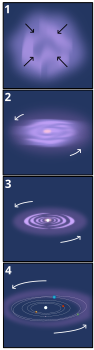
\includegraphics[height=0.82\textheight,keepaspectratio]{solar_nebula_stages}
    \source{Wikimedia, public domain}

    \column{0.75\textwidth}
    Four key stages, from top to bottom:
    \vskip8pt
    \begin{enumerate}
      \item \textbf{Cloud collapse:} a cold, dense molecular cloud fragments and contracts under self-gravity
      \item \textbf{Protoplanetary disk:} conservation of angular momentum flattens the infalling gas into a rotating disk
      \item \textbf{Disk substructure:} dust settles and concentrates into rings; streaming instability builds planetesimals
      \item \textbf{Mature system:} runaway and oligarchic growth, followed by giant impacts, produce the planets on stable orbits
    \end{enumerate}
    \vskip8pt
    Total timescale: $\sim$100~Myr from first collapse to a settled planetary system.
  \end{columns}
\end{frame}


% ── Break ───────────────────────────────────────────────────
\breakslide

% ════════════════════════════════════════════════════════════
\sectionimage{saturn_rings}{Saturn's rings, Cassini (2009). Credit: NASA/JPL/SSI}
\section{Kepler's Laws \& Orbital Elements}
% ════════════════════════════════════════════════════════════

% ── Kepler's three laws ────────────────────────────────────
\begin{frame}{Kepler's Three Laws}
  \begin{enumerate}
    \item \textbf{Law of ellipses:} Each planet orbits the Sun on an \textbf{ellipse} with the Sun at one focus.
    \vskip6pt
    \item \textbf{Equal areas:} A line from planet to Sun sweeps \textbf{equal areas in equal times}.\\
    $\Rightarrow$ faster at perihelion, slower at aphelion
    \vskip6pt
    \item \textbf{Harmonic law:}
    $$P^2 = \frac{4\pi^2}{G(M_1 + M_2)}\,a^3$$
    Connects period $P$ to semi-major axis $a$ and total mass.
  \end{enumerate}
  \vskip4pt
  Newton showed: \textbf{all three follow from universal gravitation}.
\end{frame}

% ── Kepler's laws diagram ─────────────────────────────────
\begin{frame}{Visualising Kepler's Laws}
  \centering
  
\includegraphics[width=0.85\textwidth,height=0.70\textheight,keepaspectratio]{kepler_laws}
  \source{Hankwang, CC BY 2.5}
  \vskip4pt
  {\small Elliptical orbit (left), equal areas (centre, shaded regions have equal area), and the period--semi-major axis relation (right).}
\end{frame}

% ── Orbital elements ──────────────────────────────────────
\begin{frame}{Six Orbital Elements}
  \begin{columns}[c]
    \column{0.38\textwidth}
    \centering
    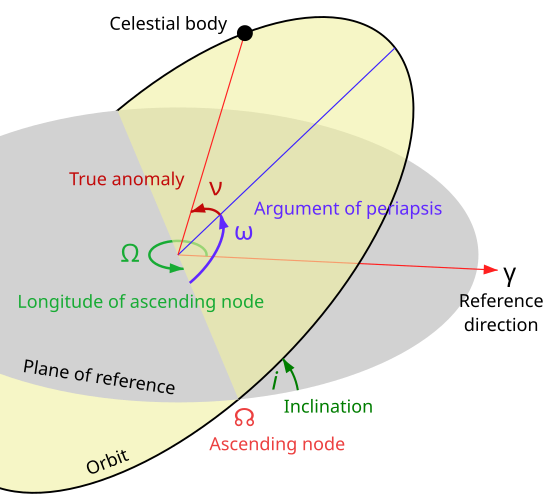
\includegraphics[width=\linewidth,height=0.65\textheight,keepaspectratio]{orbital_elements}
    \source{Lasunncty, CC BY-SA 3.0}

    \column{0.58\textwidth}
    \small
    \begin{tabular}{l c l}
      \toprule
      \textbf{Element} & \textbf{Symbol} & \textbf{Controls} \\
      \midrule
      Semi-major axis & $a$ & Size \\
      Eccentricity & $e$ & Shape \\
      Inclination & $i$ & Tilt \\
      Long.\ asc.\ node & $\Omega$ & Twist \\
      Arg.\ perihelion & $\omega$ & Orientation \\
      True anomaly & $\nu$ & Position \\
      \bottomrule
    \end{tabular}
    \vskip6pt
    First five $=$ orbit shape \& orientation.\\
    Sixth $=$ where the body is now.
  \end{columns}
\end{frame}

% ── Two-body problem ──────────────────────────────────────
\begin{frame}{The Two-Body Problem}
  Two masses $m_1$, $m_2$ interacting through gravity:
  \vskip6pt
  \begin{itemize}
    \item Reduces to \textbf{reduced mass} $\mu = m_1 m_2 / (m_1 + m_2)$ in central field of $M = m_1 + m_2$
    \item Total orbital energy:
    $$E = \frac{1}{2}\mu v^2 - \frac{G m_1 m_2}{r}$$
    \item Fundamental result: energy depends \textbf{only on $a$}:
  \end{itemize}
  \vskip4pt
  \keyresult{$$E = -\frac{G m_1 m_2}{2a}$$}
  \vskip4pt
  Same $a$ $\rightarrow$ same energy, regardless of eccentricity.
\end{frame}


% ════════════════════════════════════════════════════════════
\sectionimage{jupiter}{Jupiter, Hubble (2014). Credit: NASA/ESA/A.~Simon}
\section{Blackboard Derivation: Vis-Viva Equation}
% ════════════════════════════════════════════════════════════

% ── Setup ──────────────────────────────────────────────────
\begin{frame}{Deriving the Vis-Viva Equation}
  \textbf{Goal:} Find the speed $v$ at any distance $r$ in an orbit with semi-major axis $a$.
  \vskip10pt
  \textbf{Starting point:} Total energy is conserved and equals $E = -GMm/(2a)$.
  \vskip8pt
  At any point on the orbit:
  $$\frac{1}{2}mv^2 - \frac{GMm}{r} = -\frac{GMm}{2a}$$
  \vskip6pt
  where $M$ is the central mass ($m \ll M$).
\end{frame}

% ── Derivation step 1 ────────────────────────────────────
\begin{frame}{Step 1: Evaluate at Perihelion \& Aphelion}
  At perihelion ($r_p = a(1-e)$) and aphelion ($r_a = a(1+e)$):
  $$\frac{1}{2}mv_p^2 - \frac{GMm}{a(1-e)} = \frac{1}{2}mv_a^2 - \frac{GMm}{a(1+e)}$$
  \vskip8pt
  Angular momentum conservation:
  $$v_p \cdot a(1-e) = v_a \cdot a(1+e)$$
  \vskip6pt
  $\Rightarrow$ $v_p / v_a = (1+e)/(1-e)$
  \vskip8pt
  Solving yields $E = -GMm/(2a)$
  \vskip4pt
  \textbf{Key insight:} Energy depends only on $a$, \textbf{not} on $e$.
\end{frame}

% ── Derivation step 2 ────────────────────────────────────
\begin{frame}{Step 2: The Vis-Viva Equation}
  Setting instantaneous energy equal to the total:
  $$\frac{1}{2}mv^2 - \frac{GMm}{r} = -\frac{GMm}{2a}$$
  \vskip6pt
  Dividing by $m/2$ and rearranging:
  \vskip6pt
  \keyresult{$$\boxed{v^2 = GM\left(\frac{2}{r} - \frac{1}{a}\right)}$$}
  \vskip8pt
  Important special cases:
  \begin{itemize}
    \item \textbf{Circular orbit} ($r = a$): $v_{\mathrm{circ}} = \sqrt{GM/a}$
    \item \textbf{Escape velocity} ($a \to \infty$): $v_{\mathrm{esc}} = \sqrt{2GM/r} = \sqrt{2}\;v_{\mathrm{circ}}$
  \end{itemize}
\end{frame}

% ── Application: Earth ────────────────────────────────────
\begin{frame}{Application: Earth's Orbital Velocity}
  \centering
  \begin{tabular}{l c c}
    \toprule
    \textbf{Point} & \textbf{Distance} $r$ & \textbf{Velocity} \\
    \midrule
    Perihelion & $a(1-e) = 1.471 \times 10^{11}$~m & $v_p = 30.3$~km\,s$^{-1}$ \\
    Aphelion   & $a(1+e) = 1.521 \times 10^{11}$~m & $v_a = 29.3$~km\,s$^{-1}$ \\
    Mean       & $a = 1.496 \times 10^{11}$~m       & $\bar{v} = 29.8$~km\,s$^{-1}$ \\
    \bottomrule
  \end{tabular}
  \vskip10pt
  Nearly circular orbit ($e = 0.017$) $\rightarrow$ only $\pm 0.5$~km\,s$^{-1}$ variation.
\end{frame}

% ── Application: Halley ──────────────────────────────────
\begin{frame}{Application: Halley's Comet}
  Halley: $a = 17.8$~AU, $e = 0.967$ (extreme eccentricity)
  \vskip8pt
  \centering
  \begin{tabular}{l c c}
    \toprule
    \textbf{Point} & \textbf{Distance} & \textbf{Velocity} \\
    \midrule
    Perihelion & 0.586~AU & 54.6~km\,s$^{-1}$ \\
    Aphelion   & 35.1~AU  & 0.91~km\,s$^{-1}$ \\
    \bottomrule
  \end{tabular}
  \vskip10pt
  \begin{itemize}
    \item Races through the inner solar system at $\sim$2$\times$ Earth's speed
    \item Crawls beyond Neptune at $<$1~km\,s$^{-1}$
    \item Same total energy, just redistributed between $K$ and $U$ along the orbit
  \end{itemize}
\end{frame}


% ════════════════════════════════════════════════════════════
\sectionimage{jupiter}{Jupiter, Hubble (2014). Credit: NASA/ESA/A.~Simon}
\section{Orbital Resonances \& Tidal Forces}
% ════════════════════════════════════════════════════════════

% ── Mean-motion resonances ─────────────────────────────────
\begin{frame}{Mean-Motion Resonances}
  \begin{itemize}
    \item \textbf{$p$:$q$ resonance}: inner body completes $p$ orbits per $q$ of the outer body
    \item Gravitational kicks add up coherently $\rightarrow$ can stabilise \textbf{or} destabilise
  \end{itemize}
  \vskip6pt
  \centering
  \small
  \begin{tabular}{l l l}
    \toprule
    \textbf{Resonance} & \textbf{Bodies} & \textbf{Effect} \\
    \midrule
    3:2 & Pluto--Neptune & Protects Pluto from close encounters \\
    Near 5:2 & Jupiter--Saturn & ``Great inequality'' \\
    2:1 & Asteroid belt gaps & Kirkwood gaps (destabilising) \\
    1:1 & Jupiter Trojans & Co-orbital at L4, L5 \\
    \bottomrule
  \end{tabular}
\end{frame}

% ── Laplace resonance ──────────────────────────────────────
\begin{frame}{The Laplace Resonance}
  The Galilean moons Io, Europa, Ganymede are in a \textbf{1:2:4 period ratio}:
  \vskip6pt
  \centering
  \begin{tabular}{l c c}
    \toprule
    \textbf{Moon} & \textbf{Period (days)} & \textbf{Ratio to Io} \\
    \midrule
    Io      & 1.769 & 1 \\
    Europa  & 3.551 & $\approx$2 \\
    Ganymede & 7.155 & $\approx$4 \\
    \bottomrule
  \end{tabular}
  \vskip8pt
  \begin{itemize}
    \item Maintained by tidal interactions with Jupiter
    \item \textbf{Forces non-zero eccentricities}
    \item Io's $e \approx 0.004$ drives tidal flexing $\rightarrow$ extreme volcanism (Lecture~3)
  \end{itemize}
  \vskip4pt
  \keyresult{Orbital resonances can drive geological activity billions of years after formation.}
\end{frame}

% ── Tidal forces ──────────────────────────────────────────
\begin{frame}{Tidal Forces}
  \begin{itemize}
    \item Gravity varies across an extended body $\rightarrow$ \textbf{differential force}
    \item Tidal acceleration across a moon of radius $R_s$ at distance $d$:
    $$\Delta a_{\mathrm{tidal}} \approx \frac{2 G M_p R_s}{d^3}$$
    \item Falls off as $d^{-3}$ (steeper than gravity's $d^{-2}$)
    \vskip6pt
    \item \textbf{Tidal bulges:} elongation along the line connecting the bodies
    \item If rotation $\neq$ orbital period $\rightarrow$ bulge misalignment $\rightarrow$ torque
    \item Energy dissipated as heat $\rightarrow$ \textbf{tidal heating} (Lecture~3)
  \end{itemize}
\end{frame}

% ── Tidal locking ─────────────────────────────────────────
\begin{frame}{Tidal Locking (Synchronous Rotation)}
  \begin{itemize}
    \item Tidal torque gradually slows rotation until $P_{\mathrm{rot}} = P_{\mathrm{orb}}$
    \item Same face always points toward the planet
    \item The Moon is tidally locked to Earth (same face always visible)
    \item All four Galilean moons are tidally locked to Jupiter
    \item Locking timescale: $\tau_{\mathrm{lock}} \propto d^6 / (M_p^2 R_s^3)$
  \end{itemize}
  \vskip8pt
  \begin{exampleblock}{Note}
    Tidal locking is the \textbf{equilibrium state}. Tidal heating occurs during the approach to equilibrium (or when resonances maintain eccentricity, preventing full equilibrium).
  \end{exampleblock}
\end{frame}

% ── Roche limit ───────────────────────────────────────────
\begin{frame}{The Roche Limit}
  \begin{columns}[c]
    \column{0.42\textwidth}
    \centering
    \includegraphics[width=\textwidth]{saturn_rings}
    \source{NASA/JPL/SSI (Cassini)}

    \column{0.55\textwidth}
    Inside the \textbf{Roche limit}, tidal forces exceed self-gravity:\\
    $\rightarrow$ satellites are torn apart
    \vskip6pt
    For a fluid satellite:
    $$d_R \approx 2.46\, R_p \left(\frac{\rho_p}{\rho_s}\right)^{1/3}$$
    \vskip6pt
    For Saturn + icy satellite:\\
    $d_R \approx 126{,}000$~km $\approx 2.16\,R_{\mathrm{Saturn}}$
    \vskip4pt
    Saturn's main rings extend from 67,000 to 137,000~km, \textbf{mostly within the Roche limit} (the formula is approximate; rigid-body and compositional effects shift the boundary).
  \end{columns}
\end{frame}


% ════════════════════════════════════════════════════════════
\sectionimage{hot_jupiter}{Hot Jupiter (artist's concept). Credit: ESO/L.~Cal\c{c}ada}
\section{Planetary Migration}
% ════════════════════════════════════════════════════════════

% ── Planet-disk interactions ──────────────────────────────
\begin{frame}{Planet--Disk Interactions}
  \begin{itemize}
    \item Planets embedded in a disk excite spiral density waves
    \item Waves carry angular momentum away from the planet
    \item Net torque can push the planet \textbf{inward or outward}
  \end{itemize}
  \vskip8pt
  \begin{description}
    \item[Type I:] Low-mass planet ($\lesssim$ few $\Mearth$), fully embedded\\
    Migrates on $\sim$10$^5$~yr timescale (potentially too fast!)
    \item[Type II:] Massive planet ($\sim \Mjup$) opens a \textbf{gap}\\
    Migrates with the disk on viscous timescale ($\sim$10$^5$--$10^6$~yr)
    \item[Type III:] Rapid runaway migration in massive disks
  \end{description}
\end{frame}

% ── Nice model ─────────────────────────────────────────────
\begin{frame}{The Nice Model}
  \begin{columns}[c]
    \column{0.45\textwidth}
    \centering
    \includegraphics[width=\textwidth]{nice_model}
    \source{Wikimedia Commons, CC BY-SA 3.0}

    \column{0.52\textwidth}
    \begin{itemize}
      \item Giant planets formed in a \textbf{compact} configuration (5--17~AU)
      \item Jupiter--Saturn crossed 2:1 resonance $\rightarrow$ \textbf{instability}
      \item Uranus \& Neptune scattered outward
      \item Disrupted the primordial Kuiper Belt
      \item May explain the Late Heavy Bombardment
    \end{itemize}
  \end{columns}
\end{frame}

% ── Grand Tack ─────────────────────────────────────────────
\begin{frame}{The Grand Tack Hypothesis}
  \begin{enumerate}
    \item Jupiter migrated \textbf{inward} to $\sim$1.5~AU (Type~II migration)
    \item Saturn caught up, trapped in resonance
    \item Combined torques drove both planets \textbf{outward} (``tacking'')
    \item Jupiter swept through the inner solar system twice
  \end{enumerate}
  \vskip8pt
  Potentially explains:
  \begin{itemize}
    \item The small mass of Mars
    \item The compositional structure of the asteroid belt
    \item The distribution of water-bearing material in the inner solar system
  \end{itemize}
\end{frame}

% ── Evidence: hot Jupiters ─────────────────────────────────
\begin{frame}{Evidence for Migration: Hot Jupiters}
  \begin{columns}[c]
    \column{0.42\textwidth}
    \centering
    \includegraphics[width=\textwidth]{hot_jupiter}
    \source{ESO/L.~Cal\c{c}ada}

    \column{0.55\textwidth}
    \begin{itemize}
      \item Gas giants orbiting at $a \lesssim 0.1$~AU
      \item Orbital periods of just a few \textbf{days}
      \item Cannot have formed in situ (too hot, too little material)
      \item Must have formed further out and \textbf{migrated inward}
    \end{itemize}
    \vskip6pt
    \begin{alertblock}{}
      Hot Jupiters are the strongest evidence that planetary migration is real.
    \end{alertblock}
  \end{columns}
\end{frame}


% ════════════════════════════════════════════════════════════
\sectionimage{dsharp_gallery}{Protoplanetary disks, DSHARP. Credit: ALMA/ESO/NAOJ/NRAO}
\section{Recent Advances \& Outlook}
% ════════════════════════════════════════════════════════════

% ── Recent results ─────────────────────────────────────────
\begin{frame}{Recent Advances}
  \begin{itemize}
    \item \textbf{ALMA DSHARP survey:} Ring-and-gap substructure is ubiquitous; planet formation begins within 1~Myr
    \vskip4pt
    \item \textbf{Pebble accretion:} Refined models show giant planet cores must form within 1--3~Myr
    \vskip4pt
    \item \textbf{Juno at Jupiter:} Gravity data reveal a \textbf{dilute core}; heavy elements spread over inner $\sim$30--50\% of radius, not a compact nugget (Lecture~8)
    \vskip4pt
    \item \textbf{Meteorite isotopics:} New constraints on giant planet formation timescales from Hf--W and Mo isotope systematics
  \end{itemize}
\end{frame}

% ── Summary ────────────────────────────────────────────────
\begin{frame}{Summary}
  \begin{enumerate}
    \item Planets form in \textbf{protoplanetary disks} around young stars (lifetime $\sim$3--5~Myr)
    \item Dust grows to planetesimals via sticking, streaming instability, and pebble accretion
    \item Giant planets form by \textbf{core accretion}: solid core $\rightarrow$ critical mass $\rightarrow$ runaway gas capture
    \item Orbits follow Kepler's laws; the \textbf{vis-viva equation} gives speed at any point
    \item Orbital \textbf{resonances} can protect or destabilise orbits, and drive tidal heating
    \item Planets \textbf{migrate} through disk and planetesimal interactions, confirmed by hot Jupiters
  \end{enumerate}
\end{frame}

% ── Final slide ─────────────────────────────────────────────
\begin{frame}[plain,noframenumbering]
  \begin{tikzpicture}[remember picture, overlay]
    \ipscontain{title_background}
    \fill[ipsPrimary, opacity=0.70] (current page.north west) rectangle (current page.south east);
  \end{tikzpicture}
  \vfill
  \begin{center}
    {\color{white}\Large\bfseries Questions?}
    \vskip20pt
    {\color{ipsLightFill}\normalsize Next: \textbf{Lecture~3. Planetary Heat \& Energy Transport}}
    \vskip16pt
    {\color{ipsLightFill!70}\small Lecture notes: \texttt{formingworlds.github.io/IntroductionToPlanetaryScience}}
  \end{center}
  \vfill
\end{frame}

\end{document}
